\part{热学}
\chapter{热力学基础}
\section{温度}
温度是衡量冷热程度的物理量,测量温度的仪器统称为温度计 \\\\

\includegraphics[width=2.5cm]{example-image-duck}

摄氏度单位最初将一个标准大气压下,水结冰时的温度定为0摄氏度,水沸腾时的温度定为100摄氏度。可以采用一些物质特性与温度的关系(如:液体的热胀冷缩,热敏电阻变化)。但是采用不同物质来标定其他温度可能会出现一些误差。这里不展开讨论

\section{热量}
衡量热的作用大小的量称为热量,使用相同多少的燃料来加热不同多少的水,水越多温度上升的越慢,历史上将1克水升高或降低1摄氏度的热量称为1卡路里,现行的热量单位为焦耳,请看下一节热功当量。

\section{摩擦生热和热功当量}
焦耳做了几个实验,电流的热效应,热功当量实验等 \\
焦耳用砝码拉着叶轮,砝码在重力下向下移动一段距离就能做定量的功。\\
现在卡路里单位不是作为国际单位制的单位了,使用焦耳作为功、电功、热的统一单位。然而卡路里单位仍然在营养学等领域使用。

\section{热的传递}
两个物体接触后,两个物体的温度都会变化,

\begin{wrapfigure}{r}{-1cm}
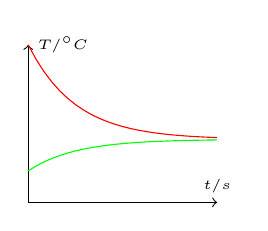
\begin{tikzpicture}[xscale=0.04, yscale=0.02,domain=0:60]
	\draw[->](0,0)--(60,0)node[left,above,font=\tiny]{$t/s$};
	\draw[->](0,0)--(0,100)node[right,font=\tiny]{$T/^\circ C$};
	\draw[color=red] plot(\x,{40+60*exp(-\x/15)});
	\draw[color=green] plot(\x,{40-20*exp(-\x/15)});
\end{tikzpicture}
\end{wrapfigure}

\begin{tabular}{c|c|c|c|c|c|c|c|c}
\hline
时间($s$) & 0 & 10 & 20 & 30 & 40 & 50 & 60 \\ \hline
温度$T_A$($^\circ C$) & 100 & 70 & 55 & 48 & 44 & 42 & 41 \\ \hline
温度$T_B$($^\circ C$) & 20 & 30 & 35 & 37 & 38 & 39 & 40 \\ \hline
温度变化率$\frac{\Delta T_A}{\Delta t}$($^\circ C$) & & -3 & -1.5 & -0.7 & -0.4 & -0.2 & -0.1 \\ \hline
温度变化率$\frac{\Delta T_B}{\Delta t}$($^\circ C$) & & 1 & 0.5 & 0.2 & 0.1 & 0.1 & 0.1 \\ \hline
\end{tabular}

观察实验记录的曲线图和数据表,曲线中A与B的温度会趋向相同。表格中A与B的温度变化率似乎有固定的比值为$3:1$,而最终温度与开始温度的差$\Delta T_A$和$\Delta T_B$的比值也为$3:1$。如果用该装置使用不同的初始温度进行实验,得到的比值不变。如果把A换成$n$倍的质量的相同物质,比例也会大$n$倍。相同质量的不同物品会有不同的比值。
